\documentclass[12pt, titlepage]{article}

\usepackage{booktabs}

\usepackage{amsmath, mathtools}
\usepackage{amsfonts}
\usepackage{amssymb}
\usepackage{graphicx}
\usepackage{colortbl}
\usepackage{xr}
\usepackage{hyperref}
\usepackage{longtable}
\usepackage{xfrac}
\usepackage{tabularx}
\usepackage{float}
\usepackage{siunitx}
\usepackage{booktabs}
\usepackage{pdflscape}
\usepackage{afterpage}
\usepackage{float}
\usepackage{fancyvrb}
\usepackage{lscape}
\usepackage{relsize}
\usepackage{listings}
\usepackage{caption}
\usepackage{subcaption}
\usepackage[english]{babel}
\usepackage[autostyle]{csquotes}


\usepackage[round]{natbib}
\hypersetup{
    colorlinks,
    citecolor=black,
    filecolor=black,
    linkcolor=red,
    urlcolor=blue
}
\usepackage[round]{natbib}

\title{Test Report: Test Plan for the Library of Linear Algebraic Equation Solver}

\author{Devi Prasad Reddy Guttapati
}

\date{\today}


%%% Comments

\usepackage{color}

\newif\ifcomments\commentstrue

\ifcomments
\newcommand{\authornote}[3]{\textcolor{#1}{[#3 ---#2]}}
\newcommand{\todo}[1]{\textcolor{red}{[TODO: #1]}}
\else
\newcommand{\authornote}[3]{}
\newcommand{\todo}[1]{}
\fi

\newcommand{\wss}[1]{\authornote{blue}{SS}{#1}}
\newcommand{\an}[1]{\authornote{magenta}{Author}{#1}}



\begin{document}




\maketitle



\pagenumbering{roman}

\begin{table}[bp]
\caption{\bf Revision History}
\begin{tabularx}{\textwidth}{p{3cm}p{2cm}X}
\toprule {\bf Date} & {\bf Version} & {\bf Notes}\\
\midrule
\today & 1.0 & Initial Draft\\

\bottomrule
\end{tabularx}
\end{table}



\tableofcontents
\listoftables
\listoffigures

\newpage



\pagenumbering{arabic}

\section{Introduction}

This document serves as the detailed Test Report for the Library of Linear Algebraic Equation Solver. It shows the detail results of the execution of Library of Linear Algebraic Equation Solver Test Plan. The requirements are described in Commonality Analysis of Library of Linear Algebraic Equation Solver. The aim of the Test Report is to show that Library of Linear Algebraic Equation Solver produces accurate and valid results.

\section{Functional Requirements Evaluation}\label{sec_fre}
\subsection{Calculation Tests}
\subsubsection{Using Gaussian Elimination: T1, T2, T3, T4}

\textbf{Test Case: T1}\\ 

Input: $A$ = (2, 3, 4, 9)
$b$ = (6, 15)

Expected Output: $x$ = (1.5, 1). This test passes.

\begin{figure}[H]
\centering
 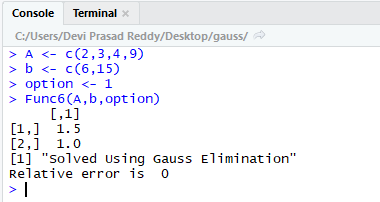
\includegraphics[width=100mm]{T1}
  \caption{T1 result.}
  \label{fig:T1}
\end{figure}

\textbf{Test Case: T2}\\

Input: $A$ = (1, 3, -2, 3, 5, 6, 2, 4, 3)
$b$ = (5, 7, 8)

Expected Output: $x$ = (-15, 8, 2). This test passes.

\begin{figure}[H]
\centering
 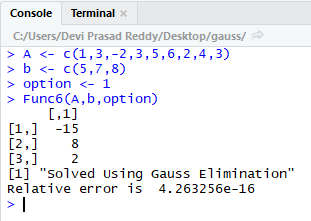
\includegraphics[width=100mm]{T2}
  \caption{T2 result.}
  \label{fig:T2}
\end{figure}

\textbf{Test Case: T3}\\

Input: $A$ = (1, 1, -2, 1, 3, -1, 2, -1, 1, 2, 2, -3, 1, 3, -3, -1, 2, 1, 5, 2, -1, -1, 2, 1, -3, -1, 2, 3, 1, 3, 4, 3, 1, -6, -3, -2)
$b$ = (4, 20, -15, -3, 16, -27)

Expected Output: $x$ = (1/3, -430/99, 313/99, 104/99, 142/33, -37/99). This test passes.

\begin{figure}[H]
\centering
 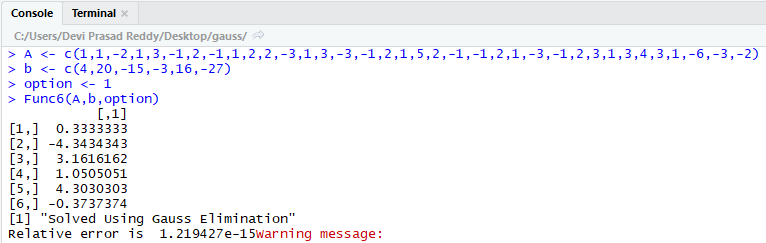
\includegraphics[width=100mm]{T3}
  \caption{T3 result.}
  \label{fig:T3}
\end{figure}

\textbf{Test Case: T4}\\

Input: $A$ = (0, 2, -1, 3, -2, 1, 3, 2, -1)
$b$ = (5, 7, 8)

Expected Output: $x$ = Singular Matrix. This test passes.

\begin{figure}[H]
\centering
 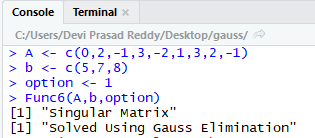
\includegraphics[width=100mm]{T4}
  \caption{T4 result.}
  \label{fig:T4}
\end{figure}


\subsubsection{Using Gauss-Jordan Elimination: T5, T6, T7, T8}

\textbf{Test Case: T5}\\ 

Input: $A$ = (2, 3, 4, 9)
$b$ = (6, 15)

Expected Output: $x$ = (1.5, 1). This test passes.

\begin{figure}[H]
\centering
 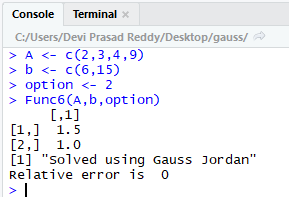
\includegraphics[width=100mm]{T5}
  \caption{T5 result.}
  \label{fig:T5}
\end{figure}

\textbf{Test Case: T6}\\

Input: $A$ = (1, 3, -2, 3, 5, 6, 2, 4, 3)
$b$ = (5, 7, 8)

Expected Output: $x$ = (-15, 8, 2). This test passes.

\begin{figure}[H]
\centering
 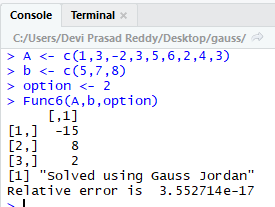
\includegraphics[width=100mm]{T6}
  \caption{T6 result.}
  \label{fig:T6}
\end{figure}

\textbf{Test Case: T7}\\

Input: $A$ = (1, 1, -2, 1, 3, -1, 2, -1, 1, 2, 2, -3, 1, 3, -3, -1, 2, 1, 5, 2, -1, -1, 2, 1, -3, -1, 2, 3, 1, 3, 4, 3, 1, -6, -3, -2)
$b$ = (4, 20, -15, -3, 16, -27)

Expected Output: $x$ = (1/3, -430/99, 313/99, 104/99, 142/33, -37/99). This test passes.

\begin{figure}[H]
\centering
 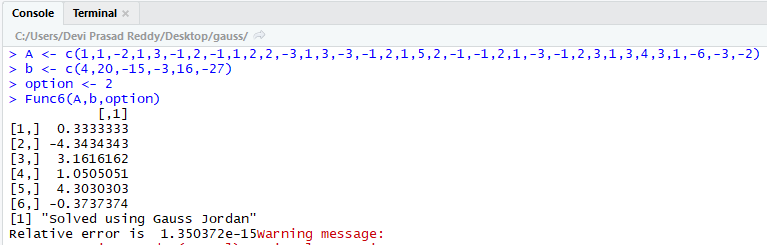
\includegraphics[width=100mm]{T7}
  \caption{T7 result.}
  \label{fig:T7}
\end{figure}

\textbf{Test Case: T8}\\

Input: $A$ = (0, 2, -1, 3, -2, 1, 3, 2, -1)
$b$ = (5, 7, 8)

Expected Output: $x$ = Singular Matrix. This test passes.

\begin{figure}[H]
\centering
 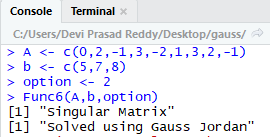
\includegraphics[width=100mm]{T8}
  \caption{T8 result.}
  \label{fig:T8}
\end{figure}


\section{Nonfunctional Requirements Evaluation}\label{sec_nfre}
\subsection{Accuracy Test}

\textbf{Test Case: T9}\\

$\epsilon_{Relative}$ will be calculated by comparing the result
obtained by Library of Linear Algebraic Equation Solver and the RStudio's optR library
functional programs by the following equation as norm

\begin{center}
 $\epsilon_\text{rel} = \text{norm} = \frac{||x_\text{R} - x_\text{LAES}||}{||x_\text{R}||}$
\end{center}

\begin{center}
\begin{tabular}{||c c||}
\hline
Test & $\epsilon_{Relative}$ \\[0.5ex]
\hline\hline
T1 & $0$\\
\hline
T2 & $4.26 \times 10^{-16}$\\
\hline
T3 & $1.21 \times 10^{-15}$\\
\hline
T5 & $0$\\
\hline
T6 & $4.26 \times 10^{-16}$\\
\hline
T7 & $1.21 \times 10^{-15}$\\
\hline

\end{tabular}
\end{center}

	
\section{Comparison to Existing Implementation}	\label{sec_cei}

In this section the comparison is done between the Library of Linear Algebraic Solver and Rstudio's optR library by unit testing and by using Functional Requirement Tests. 

\textbf{Test Case: T10}\\

The following input parameters are tested as above in Functional Requirement Tests.

\begin{itemize}
\item Test 1 (\ref{cei_t1}): $A = (2, 3, 4, 9), b = (6, 15)$
\item Test 2 (\ref{cei_t2}): $A = (1, 3, -2, 3, 5, 6, 2, 4, 3), b = (5, 7, 8)$
\item Test 3 (\ref{cei_t3}): $A = (1, 1, -2, 1, 3, -1, 2, -1, 1, 2, 2, -3, 1, 3, -3, -1, 2, 1,
5, 2, -1, -1, 2, 1, -3, -1, $
$2, 3, 1, 3, 4, 3, 1, -6, -3, -2)$

$b = (4, 20, -15, -3, 16, -27)$
\end{itemize}

\subsection{Test 1 } \label{cei_t1}

$A = (2, 3, 4, 9), b = (6, 15)$

\begin{figure}[H]
\centering
 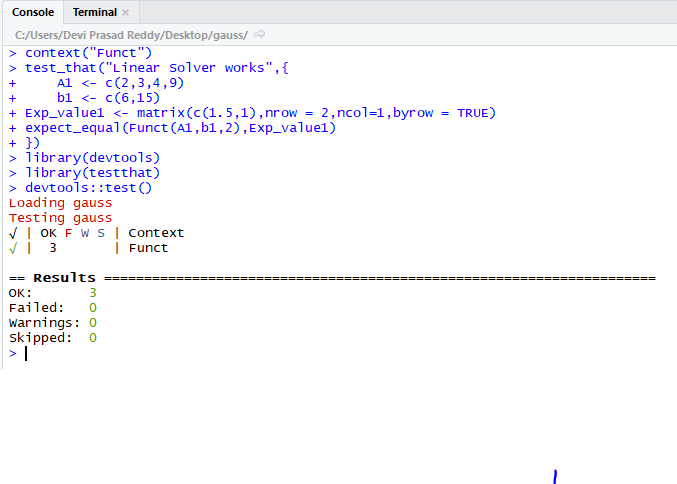
\includegraphics[width=100mm]{UT1}
  \caption{T10 Test1 result.}
  \label{fig:T9}
\end{figure}

\subsection{Test 2} \label{cei_t2}

 $A = (1, 3, -2, 3, 5, 6, 2, 4, 3), b = (5, 7, 8)$

\begin{figure}[H]
\centering
 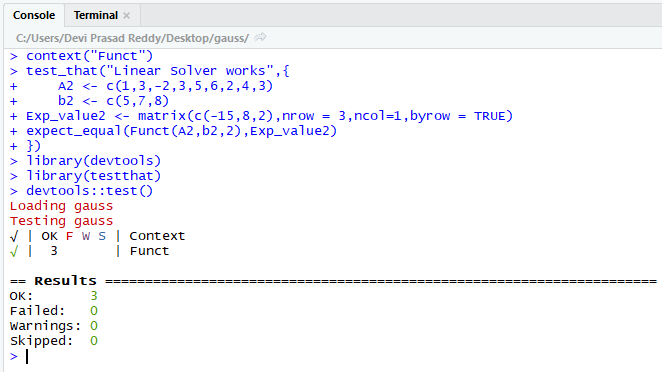
\includegraphics[width=100mm]{UT2}
  \caption{T10 Test2 result.}
  \label{fig:T10}
\end{figure}

\subsection{Test 3} \label{cei_t3}

$A = (1, 1, -2, 1, 3, -1, 2, -1, 1, 2, 2, -3, 1, 3, -3, -1, 2, 1, 5, 2, -1, -1, 2, 1,$

$-3, -1, 2, 3, 1, 3, 4, 3, 1, -6, -3, -2)$, $b = (4, 20, -15, -3, 16, -27)$

\begin{figure}[H]
\centering
 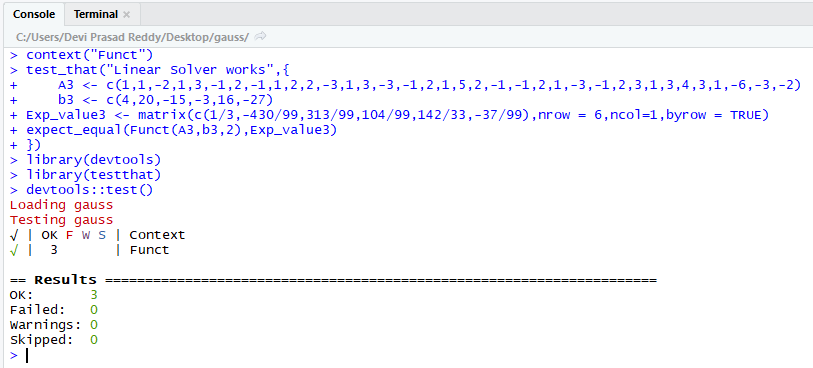
\includegraphics[width=100mm]{UT3}
  \caption{T10 Test3 result.}
  \label{fig:T11}
\end{figure}

\section{Unit Testing}

Unit testing was performed, the results and executions are similar to the Functional Requirements Evaluation which is section \ref{sec_fre} and Comparison to Existing Implementation which is section \ref{sec_cei}.

Unit testing is implemented by Rstudio's Unit Testing packages such as \enquote{devtools} and \enquote{testhat}.

\section{Changes Due to Testing}

None

\section{Automated Testing}

Automated Testing is performed in section \ref{sec_nfre} and section \ref{sec_cei}.
		
\section{Trace to Requirements}\label{sec_tracereq}

The following table shows the traceability mapping for the test cases to the requirements 
described in the Commonality Analysis.

\begin{table} [H]
  \caption{Requirements Traceability Matrix} 
\begin{tabular}{|c|p{4cm}|}
  \hline	
  \textbf{Test Number} & \textbf{CA Requirements}\\
  \hline 
   T1& IM1, C1\\ \hline
   T2& IM1, C1\\ \hline
   T3& IM1, C1\\ \hline
   T4& IM1, C1\\ \hline
   T5& IM2, C1\\ \hline
   T6& IM2, C1\\ \hline
   T7& IM2, C1\\ \hline
   T8& IM2, C1\\ \hline
   T9& IM1, IM2\\ \hline
   T10& IM1, Im2\\ \hline
   

\end{tabular}\\
\end{table}
		
\section{Trace to Modules}\label{sec_tracemodules}
The following table shows the traceability mapping for the test cases  to the
modules in the Module Guide (MG).

\begin{table} [H]
  \caption{Design Traceability Matrix}
  \label{Table:Table_Traceability_MG}  
\begin{tabular}{|c|p{8cm}|}
  \hline	
  \textbf{Test Number} & \textbf{MG Modules}\\
  \hline 
   T1& M1, M2, M3, M4, M5, M6\\ \hline
   T2& M1, M2, M3, M4, M5, M6\\ \hline
   T3& M1, M2, M3, M4, M5, M6\\ \hline
   T4& M1, M2, M3, M4, M5, M6\\ \hline
   T5& M1, M2, M3, M4, M6, M7\\ \hline
   T6& M1, M2, M3, M4, M5, M7\\ \hline
   T7& M1, M2, M3, M4, M5, M7\\ \hline
   T8& M1, M2, M3, M4, M5, M7\\ \hline
   T9& M1, M2, M3, M4, M5, M6, M7\\ \hline
   T10& M1, M2, M3, M4, M5, M6, M7\\ \hline


\end{tabular}\\
\end{table}
		

\section{Code Coverage Metrics}

The following Code Coverage figure was obtained from Rstudio's 
Code Coverage Library \enquote{Covr}. Running the test program with in-boundary
conditions, the code coverage obtained is:\\

\subsection{Using Gaussian Elimination}

\begin{figure}[H]
\centering
 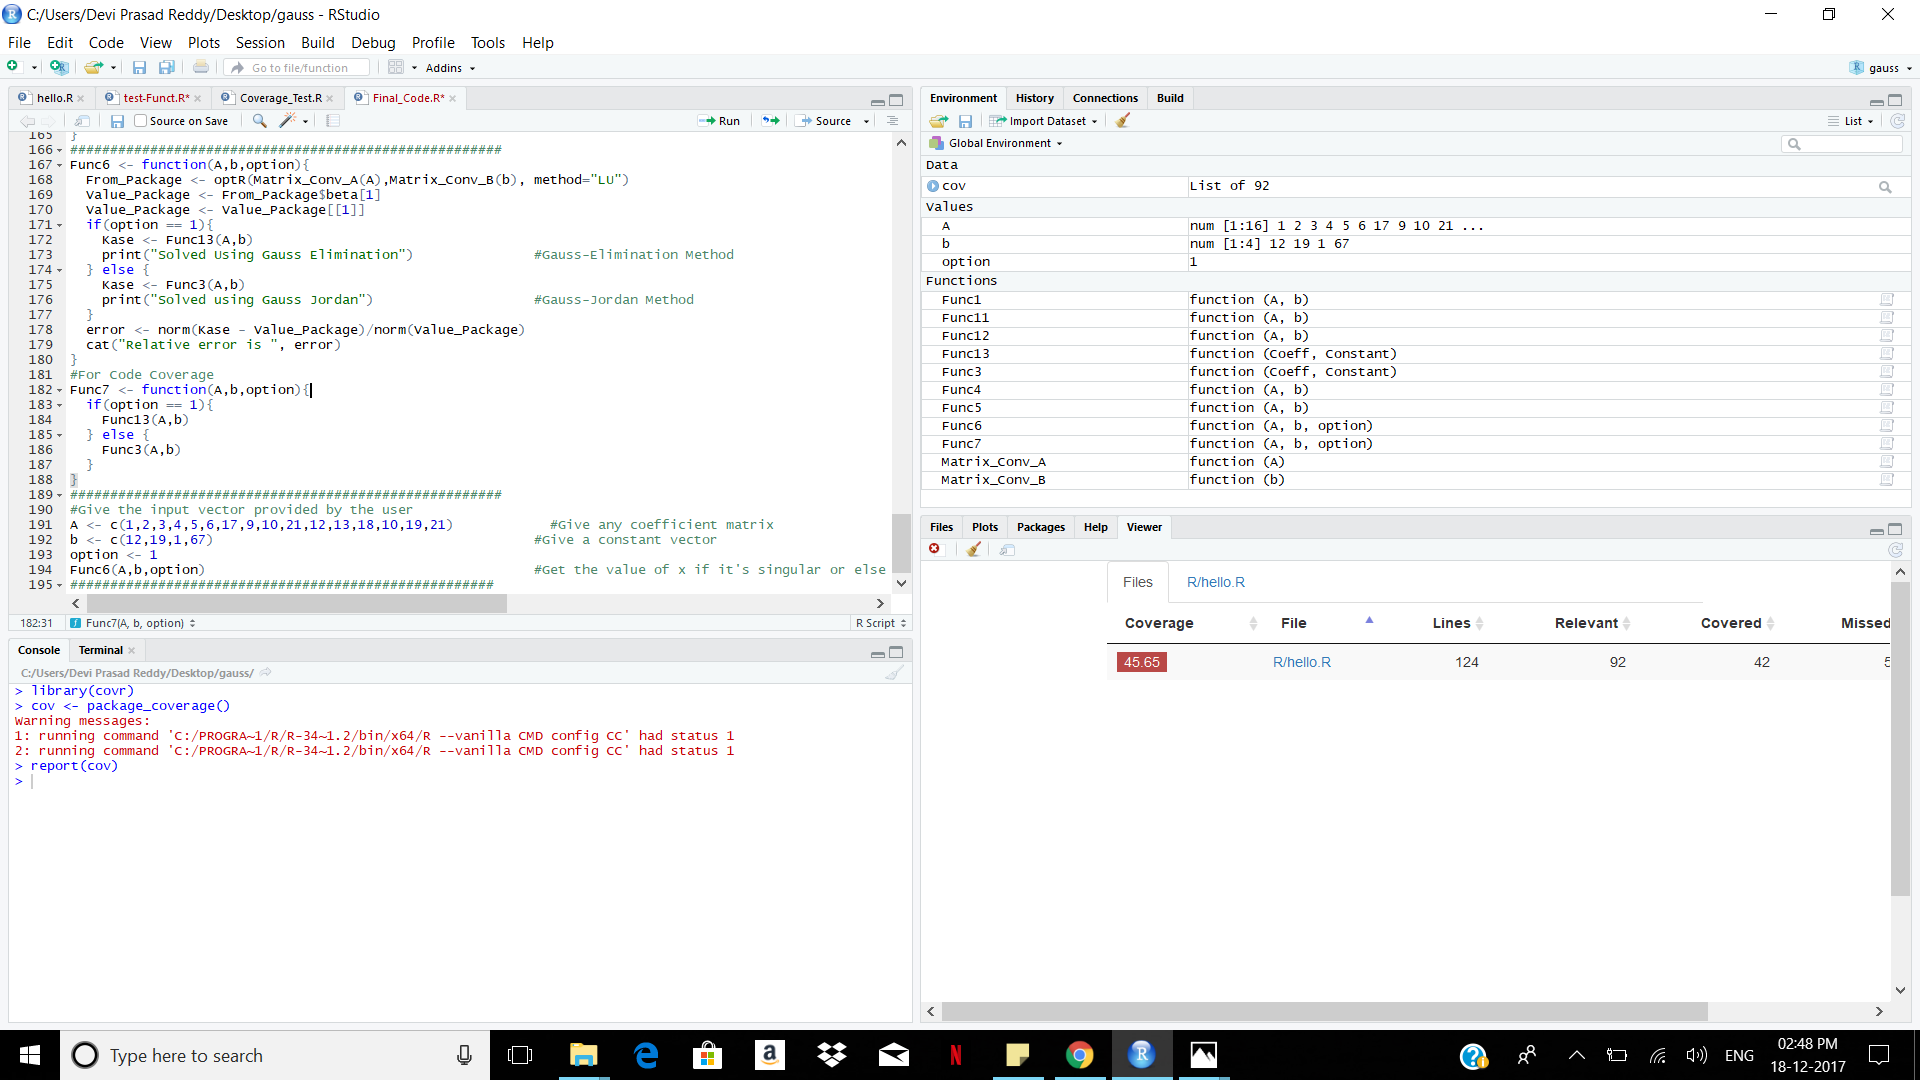
\includegraphics[width=150mm]{CV8}
  \caption{Code Coverage 1}
  \label{fig:CV8}
\end{figure}

\begin{figure}[H]
\centering
 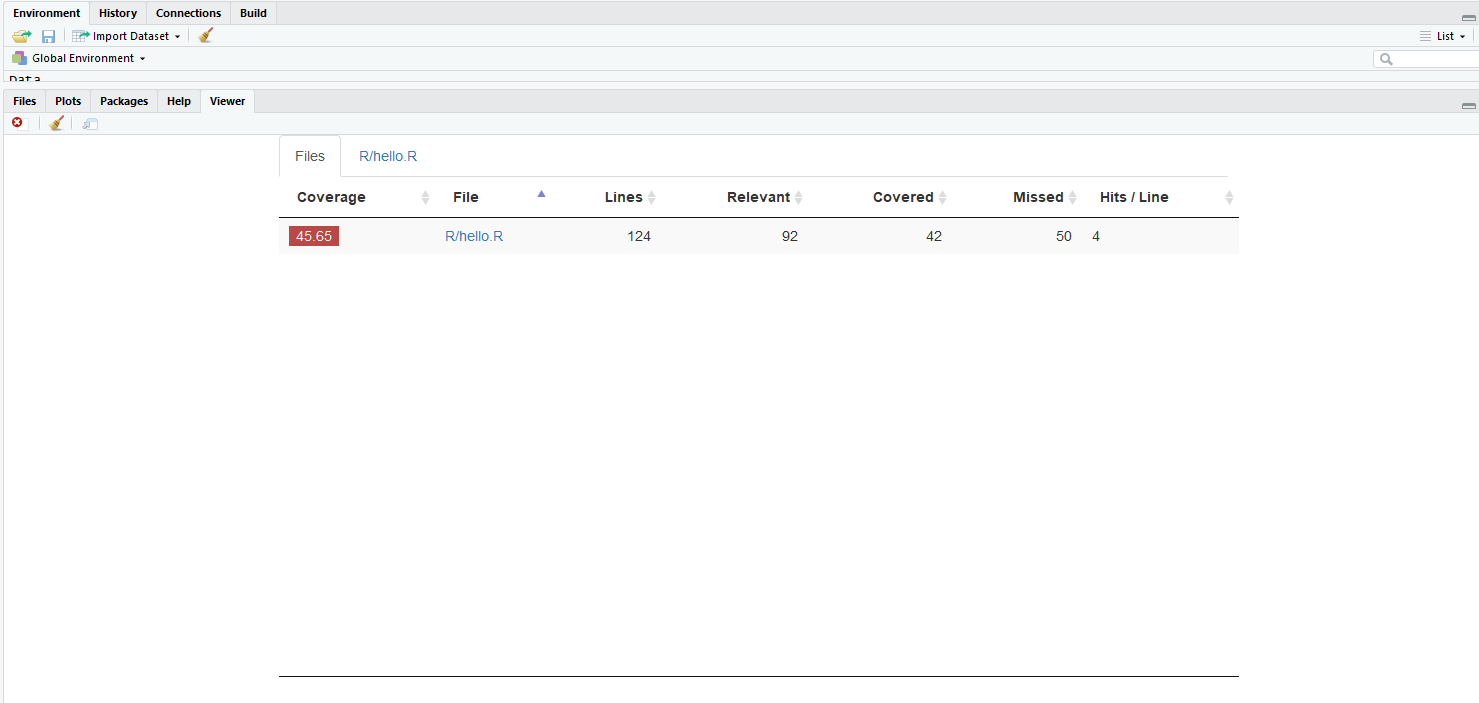
\includegraphics[width=150mm]{CV}
  \caption{Code Coverage 2}
  \label{fig:CV}
\end{figure}

\begin{figure}[H]
\centering
 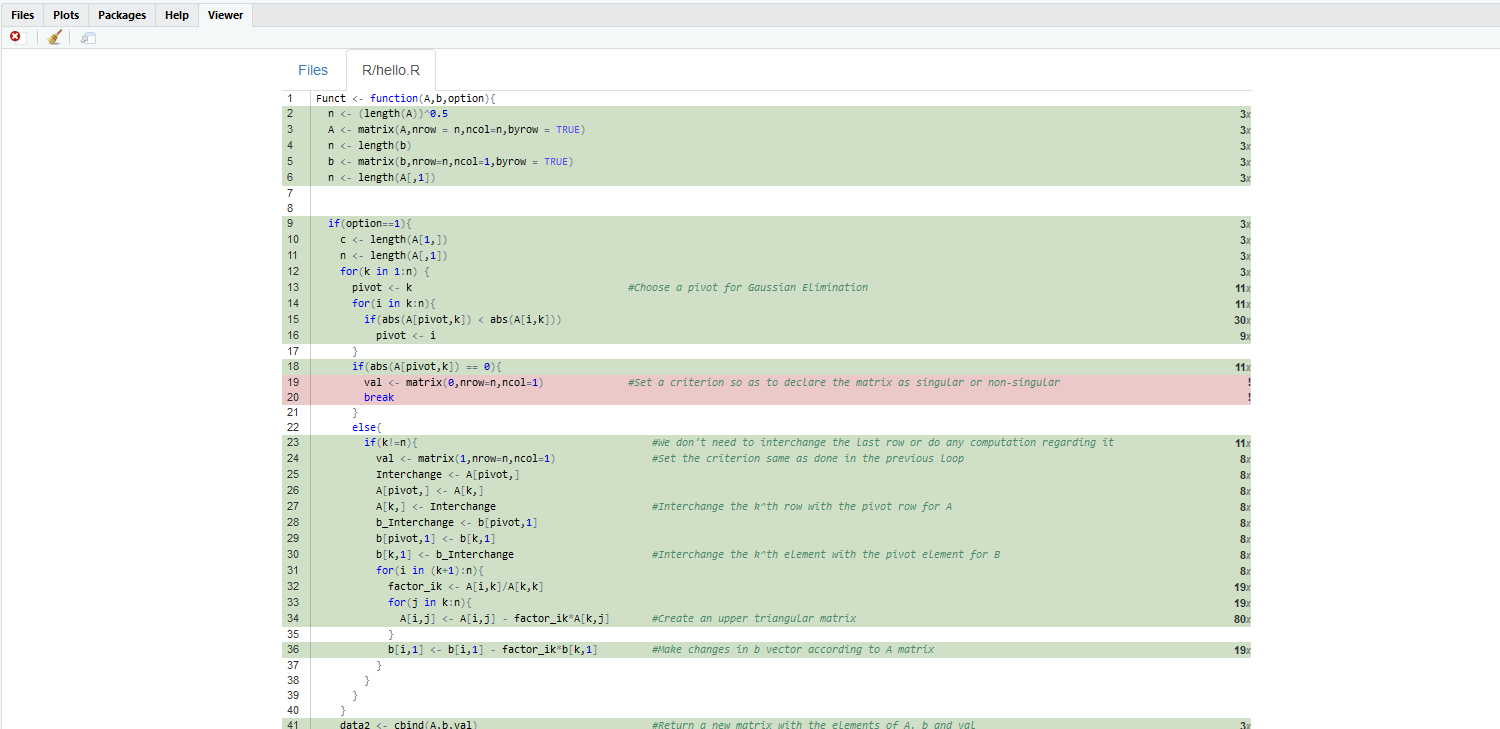
\includegraphics[width=150mm]{CV1}
  \caption{Code Coverage 3}
  \label{fig:CV1}
\end{figure}

\begin{figure}[H]
\centering
 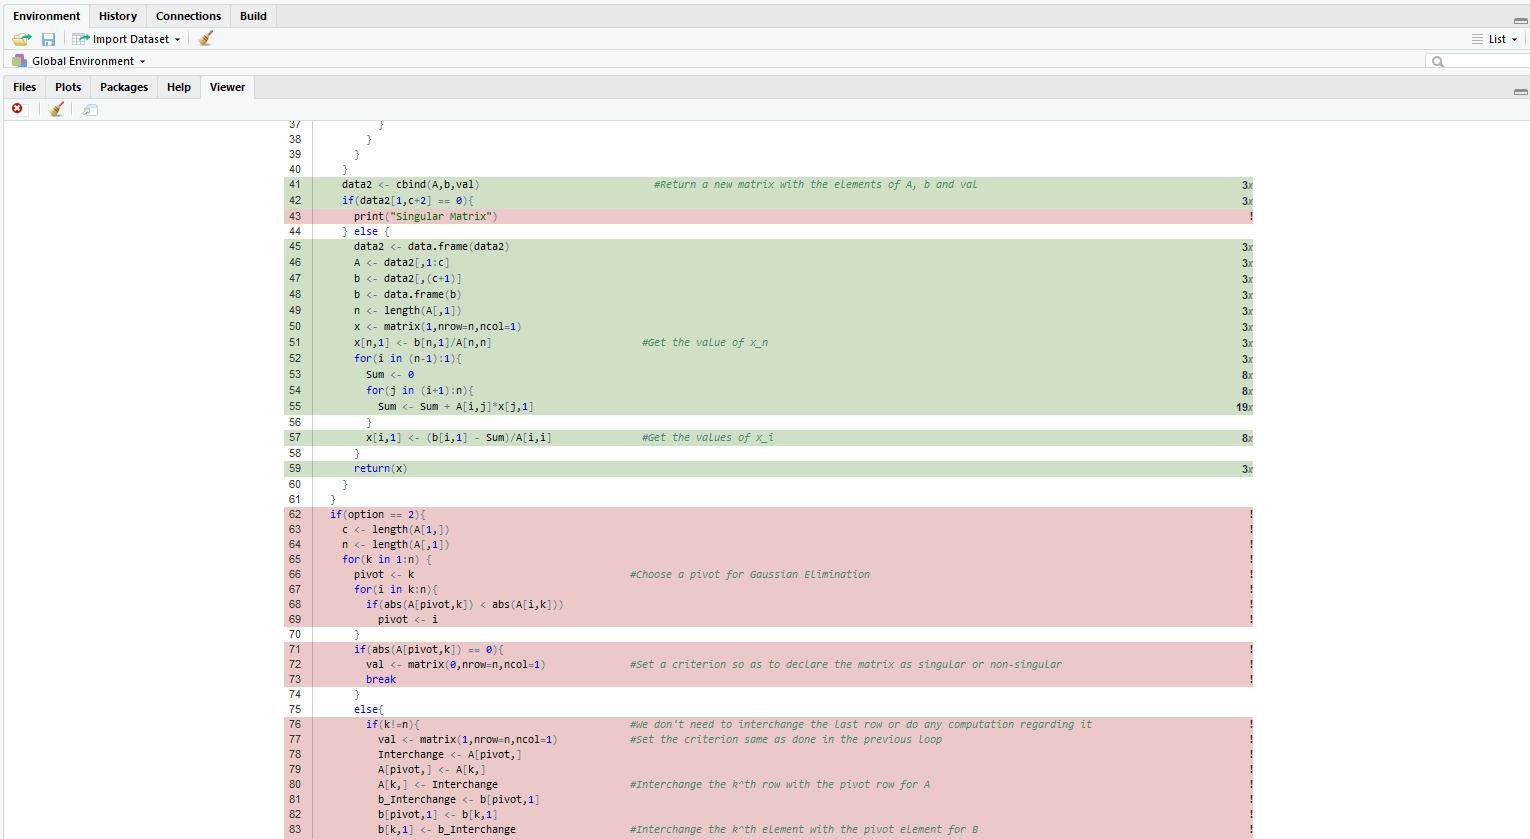
\includegraphics[width=150mm]{CV2}
  \caption{Code Coverage 4}
  \label{fig:CV2}
\end{figure}

\begin{figure}[H]
\centering
 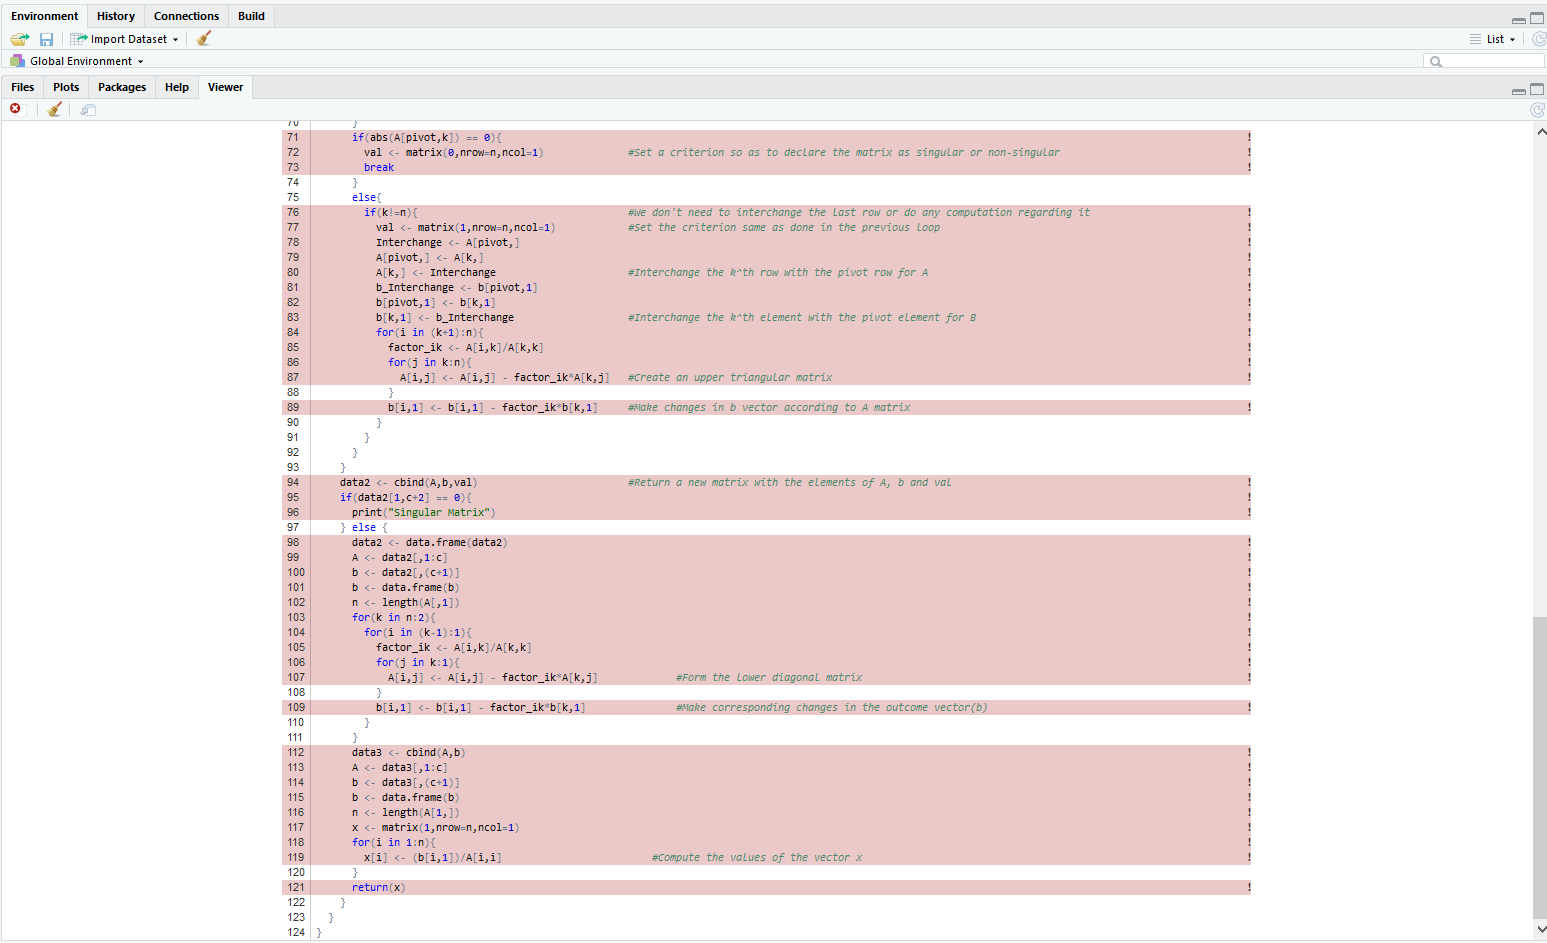
\includegraphics[width=150mm]{CV3}
  \caption{Code Coverage 5}
  \label{fig:CV3}
\end{figure}

\subsection{Using Gauss-Jordan Elimination}

\begin{figure}[H]
\centering
 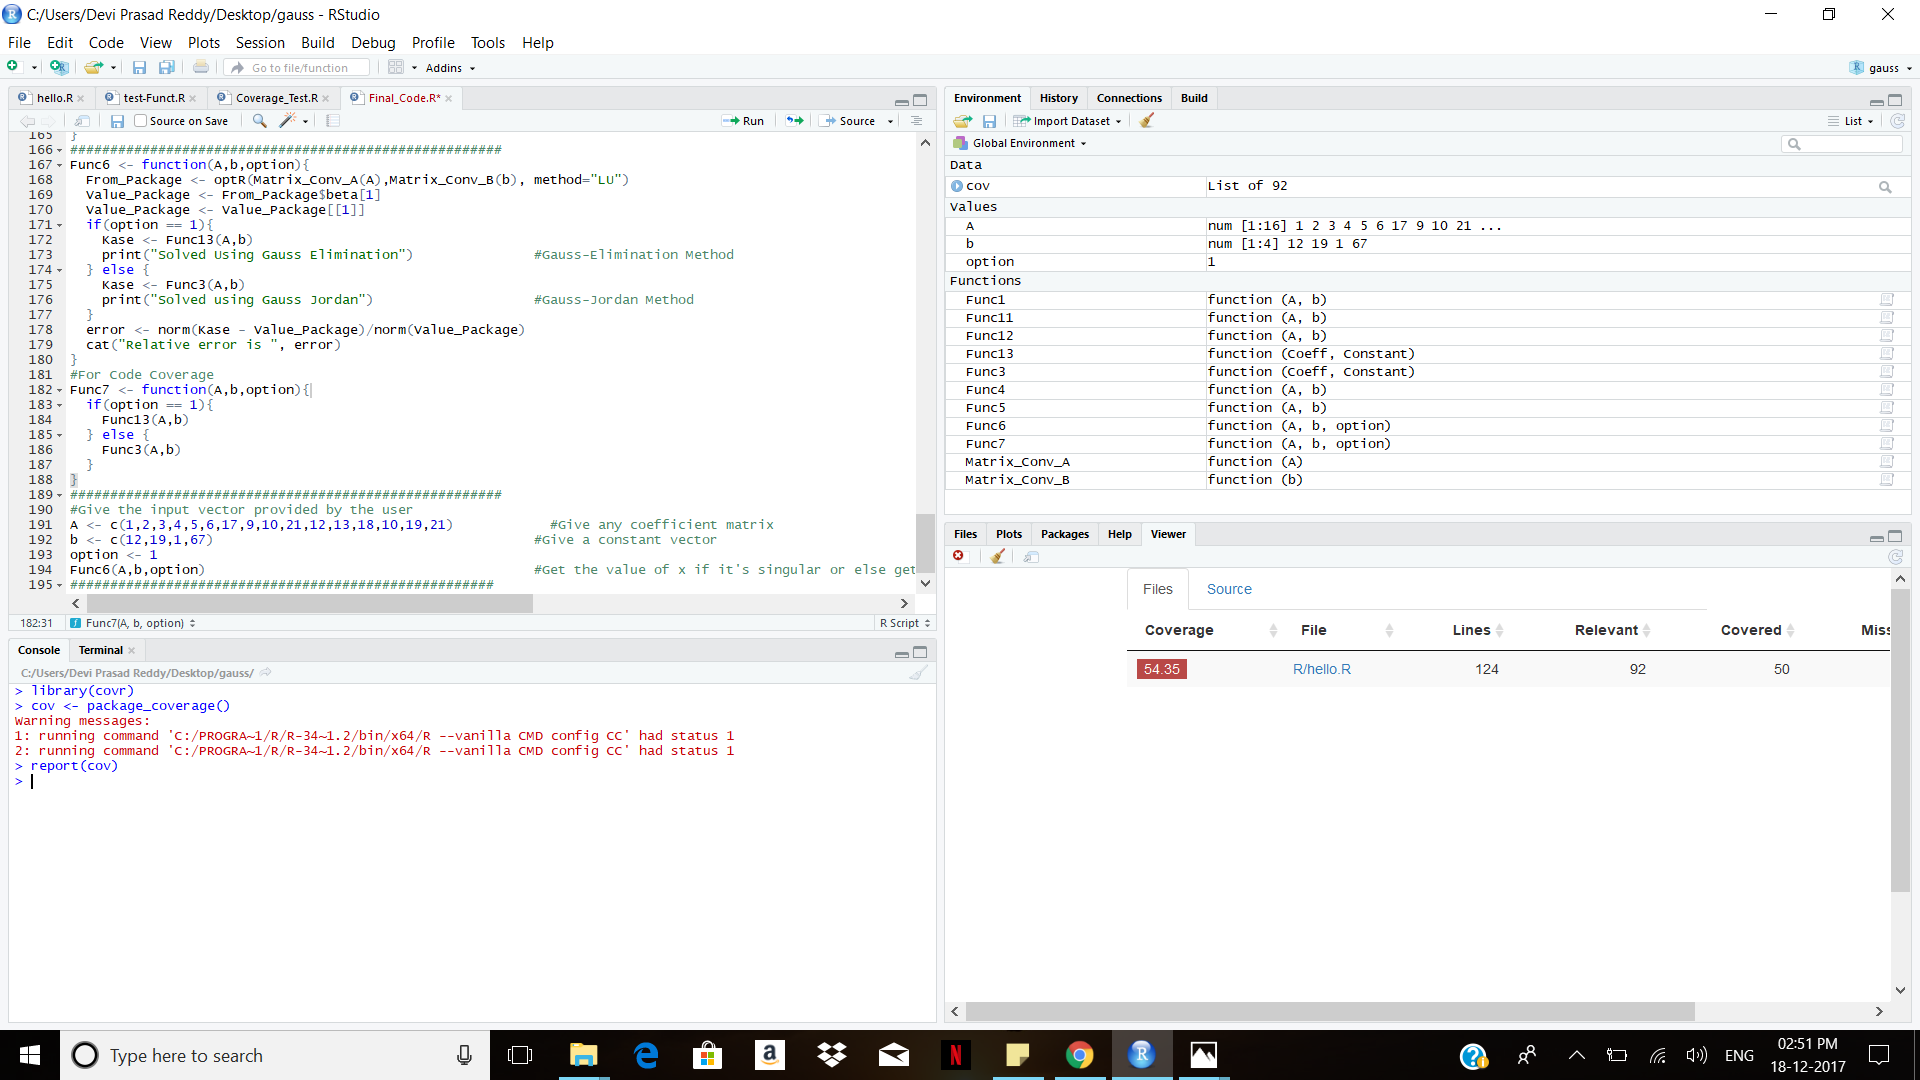
\includegraphics[width=120mm]{CV9}
  \caption{Code Coverage 6}
  \label{fig:CV9}
\end{figure}

\begin{figure}[H]
\centering
 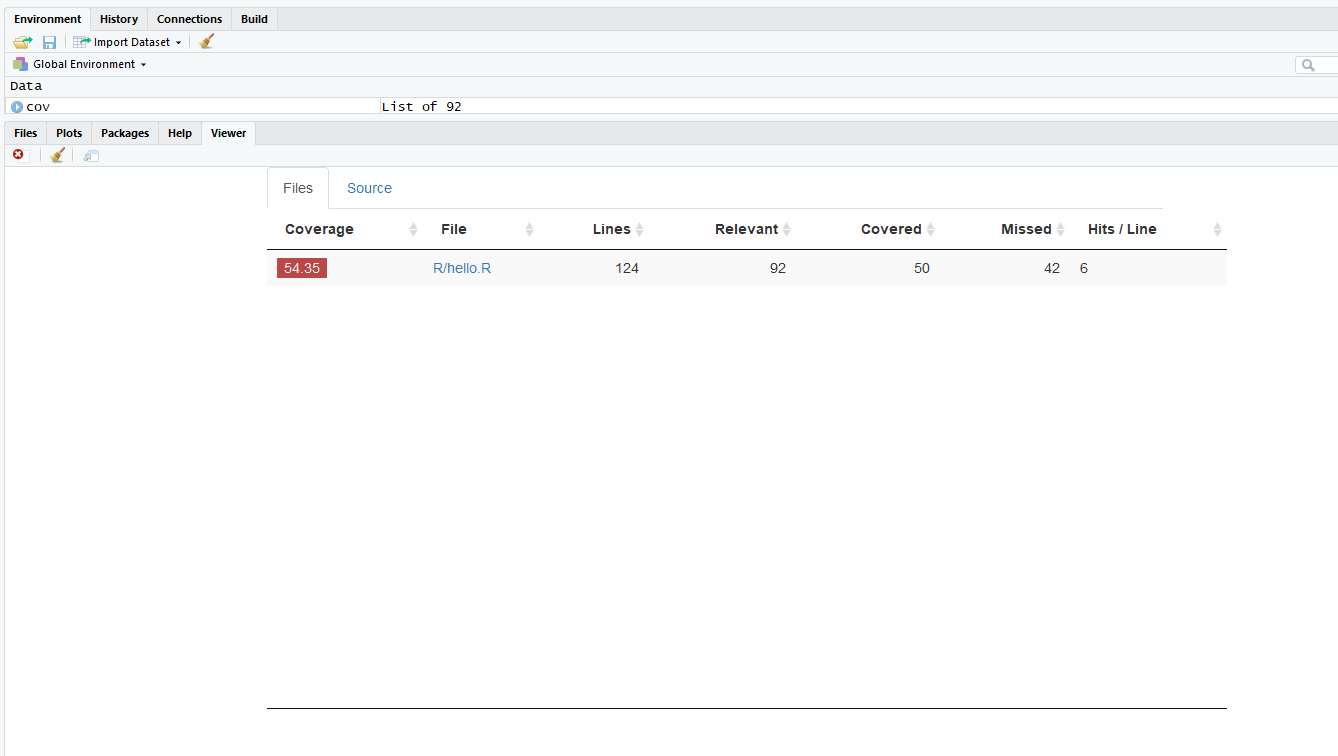
\includegraphics[width=120mm]{CV4}
  \caption{Code Coverage 7}
  \label{fig:CV4}
\end{figure}

\begin{figure}[H]
\centering
 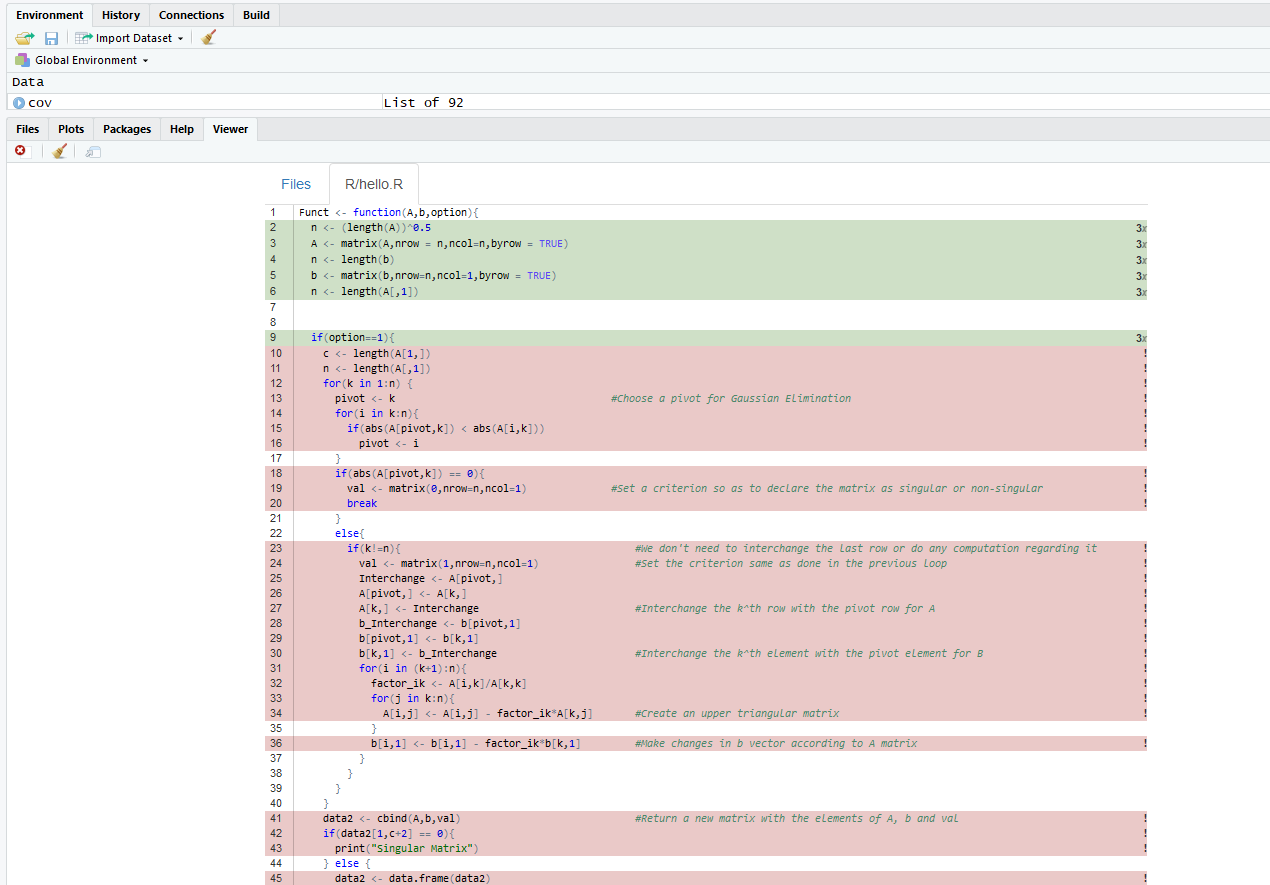
\includegraphics[width=120mm]{CV5}
  \caption{Code Coverage 8}
  \label{fig:CV5}
\end{figure}

\begin{figure}[H]
\centering
 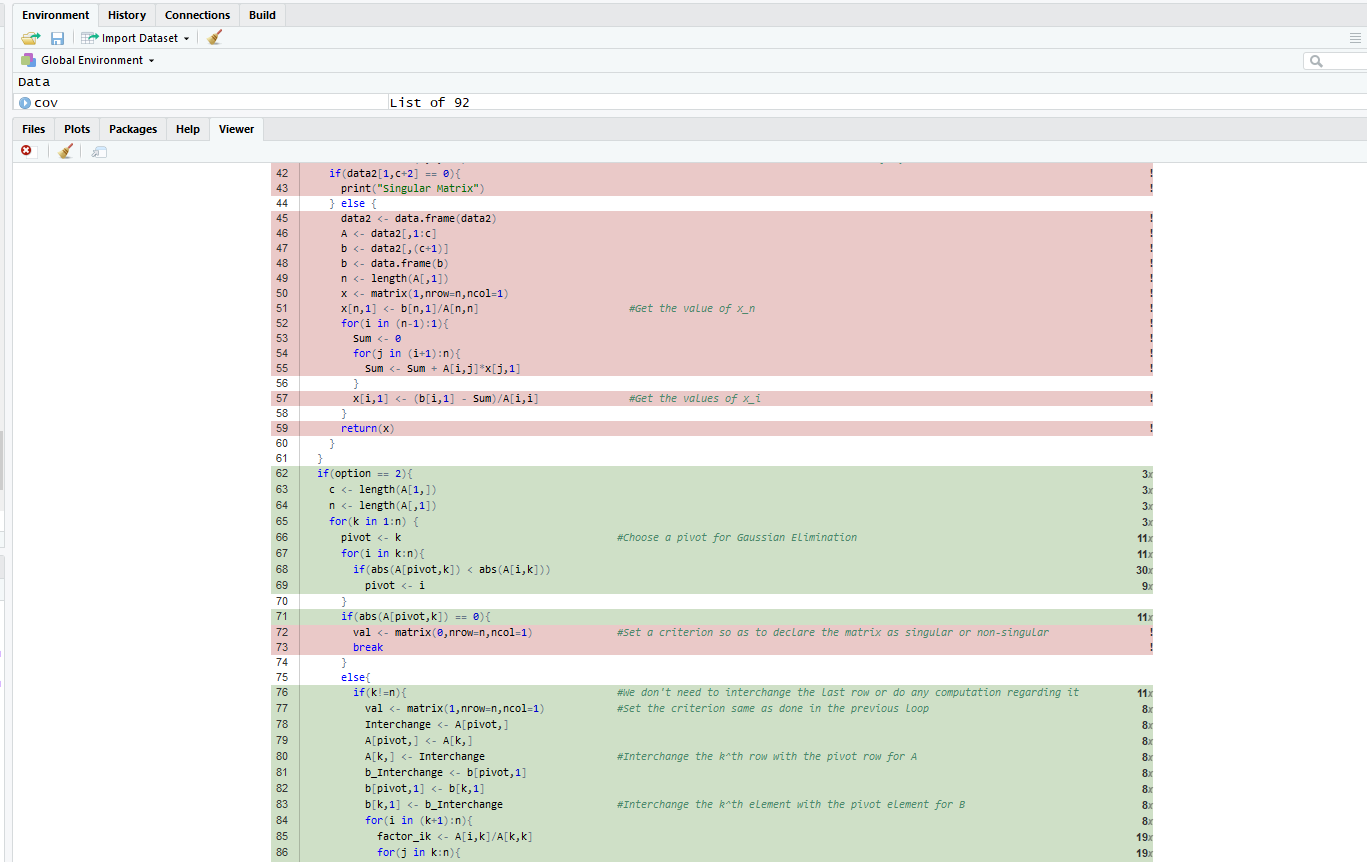
\includegraphics[width=120mm]{CV6}
  \caption{Code Coverage 9}
  \label{fig:CV6}
\end{figure}

\begin{figure}[H]
\centering
 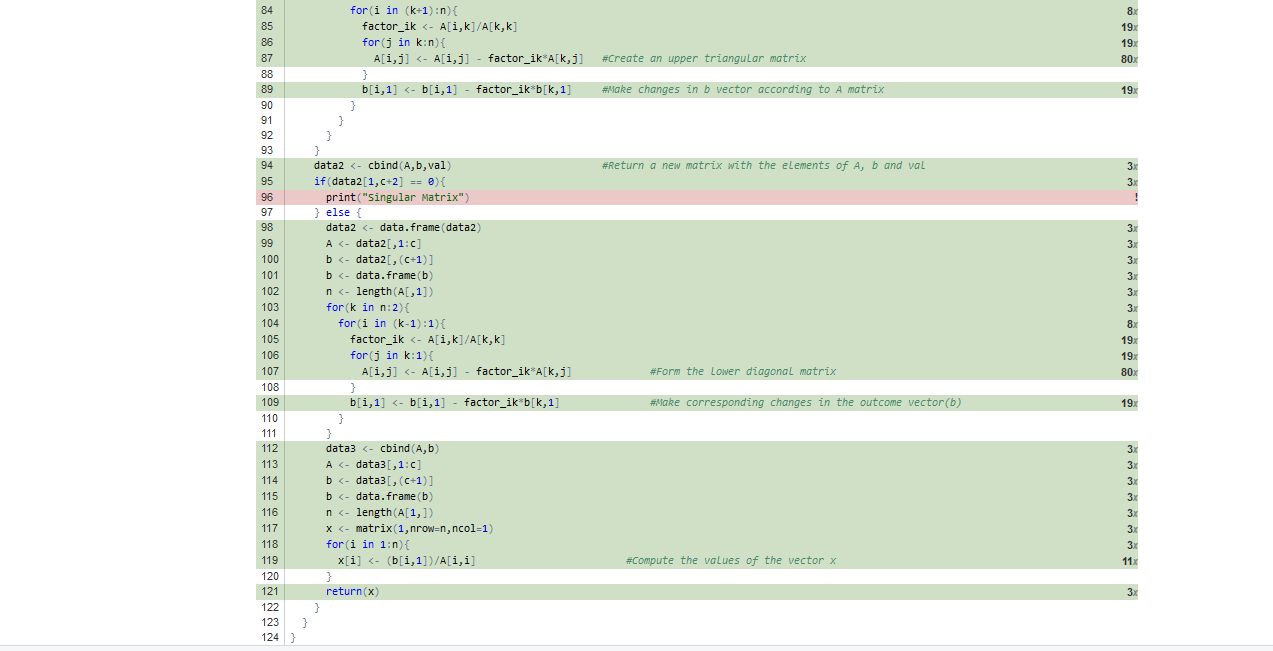
\includegraphics[width=120mm]{CV7}
  \caption{Code Coverage 10}
  \label{fig:CV7}
\end{figure}

\bibliographystyle{plainnat}

\bibliography{SRS}

\end{document}